\chapter{Sieveable: The Deep Search Engine}
\label{ch:sieveable_chapter}
As the number of mobile apps continue to proliferate in marketplaces, the need to study them at large-scale has begun to receive increased attention. 
Most of the prior work in this area is limited to a single view of the data  and lacks a  holistic view of the apps. 
In addition, data-driven systems are largely constrained by the availability of samples and efficient indexing.
This chapter presents Sieveable, a multi-view search engine for Android apps.
Sieveable enables deep searching and filtering across multiple levels: (a) Listing Details, (b) User Interface structure, (c) Manifest structure, and (d) API calls. 
Sieveable crawled and indexed more than 125,000 apps. 
It provides a query by example language to specify deep search queries. 
I discuss new findings that shed light on the potential of developing new data-driven systems based on our approach to answer different analysis questions.

\section{Introduction}

The advent of online app markets such as the Google Play Store and Apple's App Store has made it convenient for developers to publish and sell apps and users to discover, purchase and install apps. 
Together, a positive network effect has been in full force and has led to the exponential growth of the number of apps available in these online marketplaces.
These apps collectively have become an important data mining problem for many in the academia as well as in the industry.
Three domains in particular have seen significant data mining activities with respect to these apps.
First, in the commercial domain, companies have been mining listing details data such as user reviews and ratings across these apps to understand customers' opinions and preferences \cite{appbrain,apptrace}.
Second, in the user interface design domain, researchers have been mining the layouts of tens of thousands of apps to understand their design patterns \cite{Alharbi_2015_MobileHCI}.
Third, in the security domain, researchers have been mining large corpuses of apps and malwares to learn about security vulnerabilities involving permissions uses \cite{zhou_2012_SP_dissecting} and sensitive data leaks \cite{Arzt_2014_PLDI}

While research activities in these diverse domains have generated plenty of useful insights, they were often limited only to a single view of the data about each app.
Commercial data mining of mobile apps tends to focus on the public view of the app, such as the app's listing information on a marketplace's website.
The public listing information may include user reviews, ratings, app description, category, etc.
Data mining for user interface design research tends to focus on the design view of an app, such as the layout files (XML in Android) and the user interface hierarchy defined in these files (e.g., a panel containing two buttons).
Security researchers tend to pay attention to the program view of an app in the form of decompiled binaries or source code to perform programmatic analysis to understand security issues.
There is little work, if any, that has taken a holistic view of the apps encompassing these three views.

Searching and mining apps across multiple views can potentially accomplish what is currently not possible in a single view.
In UI design analysis, dynamic components created at runtime are often missed because they were defined in the program rather than in the layout files.
This shortcoming can be solved by considering both the design and program views simultaneously.
In commercial analysis, sentiment analysis of user comments in the public view can be done to understand users' opinions about the apps, but it is often difficult to link these opinions to specific features.
By incorporating the design view and program view, one can potentially establish a causal relationship between a new feature (or a bug) and the onset of certain opinions.
In security analysis, a function could be determined, through programmatic analysis, to be triggering a sensitive operation, such as sending an SMS message or taking a photo.
But it is often hard to judge if the sensitive operation is warranted from the program view alone.
By also taking a view of the design, one may examine which button may be linked to this sensitive operation and whether the button's label legitimizes such use: for example, ``Take a Picture'' for camera operations.

Multiview data mining of apps is hard to do because most of the existing system architectures for mining apps have been built for one view only.
Public view data is document-oriented where every app shares a number of common fields such as the title, ratings, and category, which can be mined from app marketplaces.
Design data is hierarchical; the layout files would specify the containment relationship between components as a tree.
Program data is highly textual as it involves a large number of names of classes, methods, and variables.
If deeper program analysis is performed, such data would involve call graphs, giving the data a network topology.
Thus, mining apps in multiple views would require an integrated infrastructure that supports document-oriented, hierarchical, textual and graphical data, and provides an easy interface to store, index, mine and analyze such data.

This chapter presents \emph{Sieveable}, a novel search infrastructure for multi-view data mining of apps on a large scale to address the needs mentioned above.
It introduces a new query language with a declarative, ``query-by-example'' syntax.
Using this language, analysts could quickly retrieve a sample from a large corpus of apps that meet certain criteria with respect to the public view, the design view, and the program view in an integrated manner.

The chapter continues as follows. An overview of our system, detail description of its implementation to enable a new multi-view analytical queries.
Prior to Sieveable, each of these analyses would take days of effort in writing custom scripts and running on a cluster \cite{Alharbi_2015_MobileHCI}.
With Sieveable, each analysis can be expressed as a query and results can be obtained in a matter of minutes.

\section{System Overview}
In this section, we describe the key requirements of our system and its core components at a high level.

\begin{table*}[t]
	\def\arraystretch{2}
	\centering
	\begin{tabular}{|>{\raggedright}p{2cm}|p{12.5cm}|}
		\hline
		\textbf{Listing \ Details \ Features} &
		package name, title, description, reviews, store URL, category, price, date published, version name, version code, target system version, ratings count, rating, content rating, creator, creator URL, install size, downloads count, permissions, what's new.\\
		\hline
		\textbf{User Interface Features} &
		layout directories, XML layout file DOM structure, drawable resources, string resources.\\
		\hline
		\textbf{Manifest Features}&
		Manifest File XML DOM structure, which includes elements such as activities, permissions, services, etc.\\
		\hline
		\textbf{Code \ Features} & 
		Framework API invocations, dependency libraries.\\
		\hline
	\end{tabular}
	\caption{Sieveable's main extracted features.}
	\label{tab:table_features}
\end{table*}

\subsection{Requirements}
We identify four main requirements that drive the technical development of the our system:
\begin{itemize}
	\item \textbf{Generalizable:}
	Given the large and diverse ecosystem of the Android platform, our search engine must be general enough to meet diverse user search goals.
	One may use the system to search for user interface design examples, API usage examples, or security permissions that protect sensitive resources.
	In order to meet various search goals, Sieveable captures powerful app's features and uses an example-based search.
	
	\item \textbf{Scalable:}
	Given the large volume of apps updated frequently, it is essential to design a scalable search engine.
	The system must be designed to be highly scalable to index billions of files. We address this goal by building a distributed search engine that can be scaled horizontally when an index becomes too large to fit a single machine.
	\item \textbf{Deep:}
	The search must be comprehensive and deep, taking into account features intrinsic to the app, such as code and UI data, as well as extrinsic features that describe the app, such as the marketplace listing details information.
	
	\item \textbf{Extensible:}
	The system must be designed to be modular and extensible to easily extend its search capabilities.
	To achieve this goal, Sieveable uses a modular plug-in architecture where each search level (e.g., UI search, code search) is a separate module that can be incorporated to the search system.
	By delegating search tasks into modules, a developer may add a new plug-in to extend the search system.
	For example, a developer may create a search plug-in for finding open source Android apps hosted on GitHub.
\end{itemize}

\subsection{Approach}
We present a novel approach that supports searching apps across multiple levels.
Our approach consists of four main steps: data collection, features extraction, features indexing, and a language specification for performing search queries.

\subsubsection{Data Collection}
We download the Android Application Package (APK) file for apps from the official marketplace, Google Play Store.
For each APK file we download and add to the dataset, a web crawler is run to obtain its listing details web page.
Next, we parsed the listing details HTML page to extract store listing values.
In order to expose the app's UI and code structure, we run a reverse-engineering tool to decompile it, which results in a directory tree of app files that make up the app. 
With more than one year effort, we manged to collect 125,306 apps with multiple versions\footnote{Note that sometimes the crawler was down, so it may have missed a number of updates.}.

\subsubsection{Features Extraction}
Once an app is downloaded and decoded, we run a set of tools to extract features at four levels:
a) Listing details level: it includes information defined in the app's marketplace listing web page.
b) User interface level: it includes all layout related files.
c) Manifest level: it includes additional internal information that describes the app.
d) Source code level: it includes all API calls invoked by the app.
All extracted features are listed in Table~\ref{tab:table_features}.

\subsubsection{Features Indexing}
When app features are extracted, we store and index them in scalable data stores to support efficient execution of search queries.
Sieveable comprises four main data collections: listing details, user interface, Manifest, and source code.
These collections are stored in different data stores and use different indexing strategies:
1) Listing details features are stored in a document oriented database.
We use text indices on specific fields (description, what's new section, reviews, and title).
2) User interface: we use a structural index that keeps track of all DOM elements' relationships (parent/child and ancestor/descendant).
3) Manifest features: we index DOM elements and their attributes.
4) Code: we use a text index to support search of invoked API methods.

\subsubsection{Query Language Specification}
\underline{\textbf{Query Syntax:}}
Sieveable uses a SQL-like declarative query syntax. The syntax is composed of three main clauses:
\begin{itemize}
	\item \textit{MATCH} The app to match. 
	\item \textit{WHERE} The search condition.
	\item \textit{RETURN} The results to return.
\end{itemize}
Example:
\begin{minted}{xml}
	MATCH app
	WHERE
	    <LinearLayout>
	       <Button/>
	    </LinearLayout>
	RETURN app
\end{minted}
The \textit{MATCH} clause defines the apps to match for the given search conditions.
The \textit{WHERE} clause defines specific search conditions. 
A search condition in its simplest form is an example of a single listing details field, UI element, manifest element, or an API call.
Multiple search conditions can be combined together allowing for a deep search across multiple levels.
The \textit{RETURN} clause defines the subset of fields to include in the results.
Multiple levels search conditions can be added to the \textit{WHERE} clause.
For example, a search query for apps developed by \textit{Google}, have a \textit{LinearLayout} with a child \textit{Button}, use the SEND\_SMS permission, and call the takePicture API call, will look like:
\begin{minted}{xml}
	MATCH app
	WHERE
    	<developer>Google Inc.</developer>
	    <LinearLayout>
	       <Button/>
     	</LinearLayout>
     	<uses-permission android:name="android.permission.SEND_SMS"/>
     	<code class="android.hardware.Camera" method="takePicture"/>
	RETURN app
\end{minted}

\underline{\textbf{Query Parser}}
When a query is submitted to Sieveable, it parses the search condition parts to determine their query levels (listing, UI, manifest, and code).
Sieveable maintains a set of dictionaries to lookup and extract search condition parts by their levels.
In particular, it maintains three dictionaries: a predefined set of listing details fields, and a set of manifest XML elements, and a single XML element named code for code related queries.
If an XML element in the query condition is not defined in any of the dictionaries, we consider it as a UI search element.
For example, in the previous search query, Sieveable parses the \textit{WHERE} clause part and groups the query parts by their levels. This results in four query parts: a) listing details query for the \texttt{<developer>} tag, b) manifest query for the \texttt{<uses-permissions>} tag, c) code query for the \texttt{<code>} tag, and UI query for the remaining elements (LinearLayout and its child). Sieveable sends these query parts to the query executor.

\underline{\textbf{Query Executor}}
\begin{figure}
	\centering
	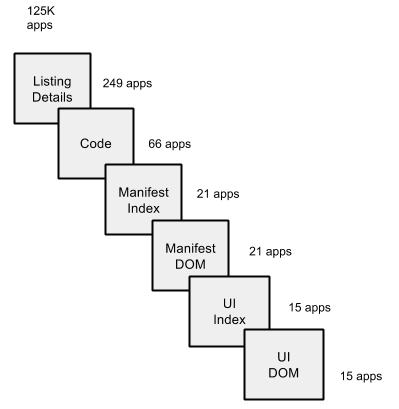
\includegraphics[scale=0.5]{figures/sieveable-deep-search/queryExecution}
	\caption{The execution sequence for a query that includes multiple level search conditions.}
	\label{fig:fig_query_execution}
\end{figure}
The query executor creates a plan for executing the received query parts.
The plan is an order of steps to query each index and data store (listing, UI, manifest, and code).
Query parts are executed by collection finder plug-ins (e.g., find by UI Index, find by UI DOM, find by code, etc.).
Collection finders return a set of app ids that matched the given query.
Sieveable computes the intersection of app ids to avoid scanning entire collections.
This also ensures that the final query results only contain ids for apps matched by all query conditions.

Figure~\ref{fig:fig_query_execution} shows the execution sequence of the aforementioned query and the number of apps scanned by each collection.
The dataset contains over 125K apps, the listing details query part is executed by the \textit{findByListing} module, which returns 249 apps developed by Google.
Next, the \textit{findByCode} module executes the code query part on the the entire collection and returns N number of apps.
Sieveable computes the intersection of the two results which becomes 66 apps.
The \textit{findByManifestIndex} module searches the Manifest index for the Manifest query part and returns N number of apps.
Sieveable computes the intersection of the two results which becomes 21 apps.
The Manifest query part is sent to the \textit{findByManifestDOM} module to match the DOM tree for those 21 apps. Since the query part contains no hierarchical structure, the DOM matcher returns the 21 apps found by the index.
Next the UI query part is sent to the index to search for apps wiht LinearLayout and child Button.
The \textit{findByUIIndex} returns N number of apps. 
Sieveable computes the intersection of the two results which becomes 15 apps.
The UI query part is sent to the \textit{findByUIDOM} module to match the DOM tree for those 15 apps which returns the final query results (15 apps).

Finally, Sieveable returns any field defined in the return statement for the matched app ids.
The query return clause includes only a single app field, so Sieveable will return an array of objects where each object contains key-value pairs for the app id, package name, and version code. Below is a part of the final query result:
\begin{minted}{javascript}
	[{
		"app": {
			"id": "com.google.android.talk-21224130",
			"packageName": "com.google.android.talk",
			"version": "21224130"
		}
	}]
\end{minted}

\section{System Implementation}
\begin{figure*}[!t]
	\centering
	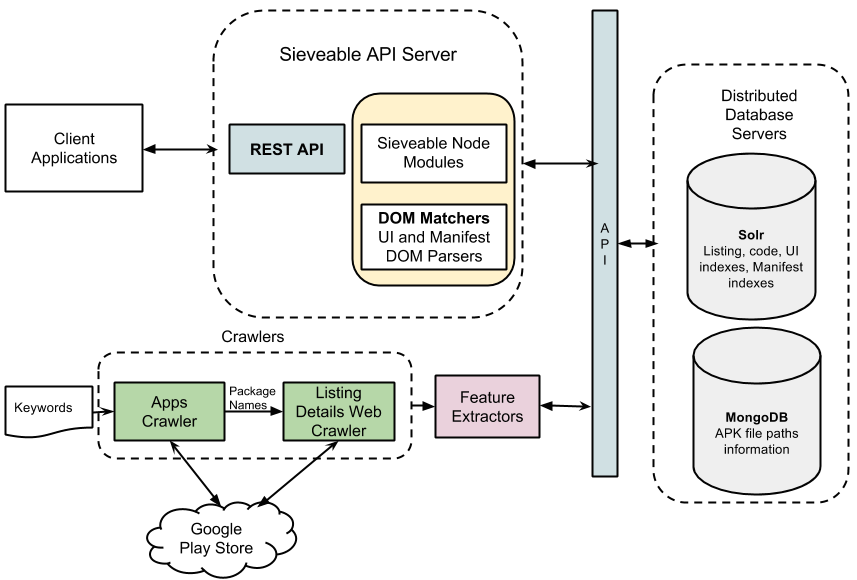
\includegraphics[width=17cm, height=10cm]{figures/sieveable-deep-search/architecture}
	\caption{Sieveable system architecture.}
	\label{fig:fig_architecture}
\end{figure*}

In this section, we discuss the technical details of designing and implementing our system. The system consists of six main components: app crawlers, feature extractors, data indexers, data store servers, DOM matchers, and a restful API (see Figure~\ref{fig:fig_architecture}).

\subsection{App Crawlers}
Sieveable features two crawlers that collect our dataset of apps: apps crawler and listing details web page crawler,
The app crawler is responsible for downloading APK files from the Google Play store.
We feed a dictionary of popular Android search keywords into the crawler.
Google has no official API for downloading APK files.
We used an unofficial API\footnote{http://github.com/Akdeniz/google-play-crawler} to collect APK files.
When an APK file is downloaded we run the Android Asset Packaging Tool (aapt) on the file to obtain its package name and version code.
We use a combination of the package name and version code as a unique identifier for each app.
APK files are stored in the file system while their ids and disk paths are stored in a MongoDB collection for fast retrieval.
Once an APK file is downloaded, we run a web crawler to fetch the most recent listing details web page of the app.
We parse the listing details fields and save them in another MongoDB collection.

\subsection{Feature Extractors}
We built a set of command line tools to extract features from the APK files.
First, we use apktool \cite{apktool}, an open-source reverse engineering tool, to decode the apps and obtain their source files.
Second, we run a custom UI parser that parses layout files and resolves any references to external resources (e.g., \texttt{android:text="@string/variable"}) or embedded layouts (using \texttt{<include/>} and \texttt{<merge/>} tags).
The parser produces a single XML file that contains the entire app UI tree, including all files.
This is especially important when performing DOM matching queries since it eliminates the need to load multiple layout files into memory when performing such queries.
Below is a snippet from an XML file generated for the YouTube app.

\begin{minted}{xml}
<App name="com.google.android.youtube" version_code="5021">
    <Directory directory_name="layout">
       <File file_name="activity_feed_item.xml">
          <RelativeLayout>
             <ImageView android:id="@id/channel_avatar"/>
           </RelativeLayout>
           ...
       </File>
    </Directory>
</App>
\end{minted}

Third, we extract all API calls from the smali files, a human readable assembly-like language for the disassembled byte code.
We save the extracted API calls in one text file per app.

\subsection{Data Indexers}
Sieveable index the extracted features and adds them to Solr indices for fast data access. We use five Solr logical indexes to index our dataset: listing index, UI tag index, ui structural index, manifest tag index, and code index.

\textbf{Indexing Listing Details:} Four listing details fields are indexed (description, title, ``what's new'', and reviews) to support text based search.

\textbf{Indexing UI data:} The extracted UI files are indexed in two Solr indices: \textit{1) Tag Index:} We extract all tag names and attributes and store them in one index document.
This index holds all tag names and their attributes.
\textit{2) Structural Index:} a suffix tree based index that stores the XML tree in a suffix array format \cite{shasha_2002_atreegrep}.
This index holds values that indicate the parent-child relationship of nodes in the XML tree. (e.g., \path{LinerLayout->Button}).
We parse the single XML UI tree file we extracted for each app and generate two text documents. The first text document contains the tag and attribute names for all UI elements (e.g., \path{EditText(android:layout_width="fill_parent")}).
We add this document to Solr and use it as the tag index.
The second generated document describes the UI tree in a suffix-tree format where each line corresponds to a root-to-leaf path for all XML elements (e.g., \path{RelativeLayout->LinearLayout->ImageButton}).
We add this document to Solr and use it as the structural index.

\textbf{Indexing Manifest data:} The extracted manifest files are indexed by their tag names and attribute values.
Unlike UI queries, Manifest queries are less structural (e.g., find \path{"android.permission.CAMERA"}).
Therefore, we use the same UI tag index method to add manifest files to the Solr Index.

\textbf{Indexing Code files}, we add the extracted invoked API calls from the smali source code files to Solr.

\subsection{Data Store Servers}
Sieveable uses three database servers: 
a) MongoDB: contains collections for listing details and downloaded APK file paths.
b) Apache Solr: contains indices for the UI tags and attributes, UI structural, Manifest attributes, and Code files.
c) Redis: a key-value data store where keys correspond to a dataset type (UI, manifest, code) and values are the unique app ids.
This is used to improve the performance of computing the intersection of the returned ids from each collection.
\subsection{DOM Matchers}

Sieveable UI and Manifest search queries are written in ``query-by-example'' syntax.
We implement a custom DOM matchers module to navigate the XML DOM tree and select DOM elements with a particular DOM structure.
The DOM matchers are written in Node.js using a jQuery like DOM manipulation library called cheerio.
While loading DOM files for complex queries is often considered expensive, the hierarchical indices we implemented significantly increased the number of potential candidates. 
However, parsing the DOM for large number of files has an inevitable memory and system resources overhead.
Therefore, Sieveable uses a configurable default limit of 10 results per a given search query.
Users can also use a streaming API to receive the entire query results.

\subsection{RESTful API}
Client applications can access Sieveable through a RESTful API. The API provides an HTTP GET request mechanism. It features a streaming based access, where it maintains a long-running request and pushes the results as they become available.
This is useful when submitting queries and asking Sieveable to return the entire result.
By streaming results, client applications do not have to wait until the query completes its execution. 
For an easy query access, Sieveable has a web client application that interacts with the RESTful API.

\section{Comparison to Prior Work}
%TODO

\section{Discussion and Future Work}
This chapter presented Sieveable, a multi-view search engine for apps on a large-scale.
It discussed the importance of searching and mining apps across multiple views.
For the first time, Sieveable can help users execute deep search queries (illustrated in Chapter \ref{ch:findings_chapter}) and apply data driven approaches with a holistic view of apps at large-scale that could yield valuable results.
This work has a number of directions for future work:

\begin{itemize}
	
	\item\underline{\textit{Deep Analysis:}} Sieveable opens up a wide opportunity to apply an in-depth analysis of mobile apps across multiple levels to investigate emergent trends in mobile apps development.
	
	\item \underline{\textit{Logical Query Operators:}} Search query conditions can be joined using OR, AND, NOT, NOR operators.
	
	\item \underline{\textit{Faceted Search:}} Applying multiple listing details filters could help users explore search results and arrange them into categories.
	
	\item\underline{\textit{Search Goals:}} Sieveable has been deployed and used in a distributed computing infrastructure.
	Releasing it to users and collecting their submitted queries could help us understand interesting search goals \cite{rose_2004_WWW_understanding} and realize new applications.
	
\end{itemize}
For more information on using Sieveable including source code access and over 100 query examples, please visit:
\url{https://github.com/sikuli/sieveable}
